\documentclass[UTF8,12pt]{ctexart}

\usepackage[margin=1in]{geometry}
\usepackage{setspace}
\usepackage{graphicx}
\usepackage{booktabs}
\usepackage{caption}
\usepackage{float}
\usepackage{hyperref}
\usepackage{xurl}
\usepackage{natbib}
\usepackage{amsmath}

\hypersetup{
  colorlinks=true,
  linkcolor=black,
  citecolor=blue,
  urlcolor=blue
}
\Urlmuskip=0mu plus 2mu\relax
\onehalfspacing

\title{教育是否提高中国成年人的收入？\\基于 CFPS 2022 的数据审计、双重稳健估计与弱工具变量诊断}
\author{实证论文}
\date{2026 年 6 月 25 日}

\begin{document}
\maketitle

\begin{abstract}
本文使用 CFPS 2022 微观数据重新考察教育是否提高中国成年人的收入。相较于传统明瑟方程，本文做了三方面改进。第一，加入完整的数据质量检查，报告样本筛选、缺失情况、异常值处理和共同支撑。第二，将核心问题从“受教育年限与收入是否相关”推进到“大专及以上教育是否提高工资收入”，并使用交叉拟合的增强逆概率加权（AIPW）估计平均处理效应。第三，检验而不是直接假定 1999 年高等教育扩招可以作为工具变量识别策略。最终分析样本为 4,699 名劳动年龄成年人。OLS 结果显示，受教育年限每增加一年，工资收入约高 8.8\%；大专及以上教育对应约 0.74 个对数点的工资优势。首选 AIPW 估计为 0.710 个对数点，稳健性估计范围为 0.669--0.773。平衡性诊断显示，权重显著降低了年龄、性别、户口、城乡、婚姻和医保等协变量差异。然而，扩招工具变量在较窄出生队列窗口中的第一阶段很弱，因此本文只将其作为诊断结果，而不将其包装为主要因果证据。总体而言，本文支持教育与收入之间存在显著正向关系，并提供了比简单 OLS 更扎实的选择性可观测条件下的处理效应估计。
\end{abstract}

\noindent\textbf{关键词：} 教育；收入；CFPS；双重稳健估计；因果推断；高等教育扩招

\section{引言}

教育是解释劳动市场收入差异的重要因素。人力资本理论认为，教育能够通过提升技能、生产率和职业匹配质量来增加收入 \citep{becker1964human, mincer1974schooling}。但是，教育并非随机分配，家庭背景、能力、地区机会和制度条件可能同时影响教育和收入，因此简单 OLS 往往只能解释为条件相关关系 \citep{card1999causal, heckman2008earnings}。

本文此前版本主要回答“教育与收入是否显著正相关”。这个问题有意义，但创新性和因果推断不足。新版论文将研究设计改为三层结构：第一，先做数据审计，说明样本如何从原始数据进入最终回归；第二，以“大专及以上教育”为处理变量，使用双重稳健 AIPW 方法估计平均处理效应 \citep{hirano2003efficient, bang2005doubly}；第三，尝试利用 1999 年高等教育扩招作为政策暴露，但根据第一阶段强度判断其是否可作为主识别策略。

因此，本文的创新并不是声称已经获得完美因果识别，而是在可用数据条件下更诚实、更扎实地推进识别：OLS 作为基准，AIPW 作为主要因果推断框架，扩招工具变量作为经过检验的辅助诊断。

\section{文献与识别思路}

本文的起点是明瑟收入方程 \citep{mincer1974schooling}。大量研究发现教育与收入正相关，但也强调 OLS 可能受到不可观测能力和家庭背景影响 \citep{card1999causal}。在中国语境下，\citet{zhang2005urban} 发现市场化改革时期城市教育回报上升，\citet{asadullah2020changing} 和 \citet{ma2021meta} 进一步说明教育回报会随时期、性别、户口、地区和部门而变化。

高等教育扩招文献为因果识别提供了重要启发。\citet{huang2022expansion} 利用高等教育扩招考察教育回报及户口差异。本文借鉴这一政策思路，但不直接假定其在 CFPS 2022 横截面中有效，而是先检验 1981 年前后出生队列是否存在足够强的教育跳跃。根据回归断点设计的实践要求 \citep{imbens2008rd, lee2010rd}，如果局部第一阶段很弱，就不应将其作为主因果证据。

本文主要使用选择性可观测条件下的 AIPW 估计。AIPW 同时结合结果模型和倾向得分模型；在条件可忽略性成立时，只要其中一个模型设定正确，估计量仍可保持一致 \citep{bang2005doubly}。由于该假设无法直接检验，本文同时报告倾向得分重叠和平衡性改善情况。

\section{数据与数据检查}

本文使用 CFPS 2022 数据 \citep{xie2015sampling, cfps2022data}。原始数据包含 9,806 个观测值。样本处理包括保留 18--64 岁成年人、要求工资收入可得、并要求核心变量完整。表 \ref{tab:flow} 展示样本筛选过程。

\begin{table}[H]
\centering
\caption{样本构造过程}
\label{tab:flow}
\begin{tabular}{lrl}
\toprule
步骤 & 样本量 & 规则 \\
\midrule
CFPS 2022 原始数据 & 9,806 &  \\
保留 18--64 岁成年人 & 7,975 & 年龄限制 \\
要求工资变量非缺失 & 4,718 & 因变量可得 \\
要求核心变量完整 & 4,699 & 最终分析样本 \\
\bottomrule
\end{tabular}

\end{table}

主要因变量为 $\ln(\mathrm{wage}+1)$。连续教育变量为受教育年限；因果估计中的处理变量为是否完成大专及以上教育。表 \ref{tab:missing} 显示，工资变量缺失是样本减少的主要来源，而多数协变量缺失比例较低。工资的 99 分位数为 300,000 元，因此稳健性检验中加入工资缩尾口径。

\begin{table}[H]
\centering
\caption{原始数据缺失情况检查}
\label{tab:missing}
\begin{tabular}{lrr}
\toprule
变量 & 缺失样本量 & 缺失比例 \\
\midrule
wage & 4,934 & 50.32 \\
educ & 1 & 0.01 \\
age\_ & 0 & 0.00 \\
gen & 0 & 0.00 \\
mar & 261 & 2.66 \\
rural & 97 & 0.99 \\
urban & 79 & 0.81 \\
health & 139 & 1.42 \\
inter & 350 & 3.57 \\
dw & 408 & 4.16 \\
asset & 926 & 9.44 \\
\bottomrule
\end{tabular}

\end{table}

\begin{table}[H]
\centering
\caption{描述性统计}
\label{tab:desc}
\begin{tabular}{lrrrrrr}
\toprule
变量 & 样本量 & 均值 & 标准差 & 最小值 & 中位数 & 最大值 \\
\midrule
年度工资收入 & 4,699 & 60594.132 & 68985.459 & 0.000 & 48000.000 & 1800000.000 \\
ln(工资 + 1) & 4,699 & 10.489 & 1.567 & 0.000 & 10.779 & 14.403 \\
受教育年限 & 4,699 & 11.006 & 4.376 & 0.000 & 12.000 & 22.000 \\
年龄 & 4,699 & 40.867 & 10.921 & 18.000 & 40.000 & 64.000 \\
男性 & 4,699 & 0.575 & 0.494 & 0.000 & 1.000 & 1.000 \\
农业户口 & 4,699 & 0.795 & 0.404 & 0.000 & 1.000 & 1.000 \\
\bottomrule
\end{tabular}

\end{table}

\begin{table}[H]
\centering
\caption{教育水平分布}
\label{tab:edu}
\begin{tabular}{lrr}
\toprule
教育类别 & 样本量 & 占比（\%） \\
\midrule
文盲 & 243 & 5.17 \\
小学 & 589 & 12.53 \\
初中 & 1,463 & 31.13 \\
高中 & 774 & 16.47 \\
大专 & 702 & 14.94 \\
本科 & 824 & 17.54 \\
硕士 & 91 & 1.94 \\
博士 & 13 & 0.28 \\
\bottomrule
\end{tabular}

\end{table}

\begin{figure}[H]
\centering
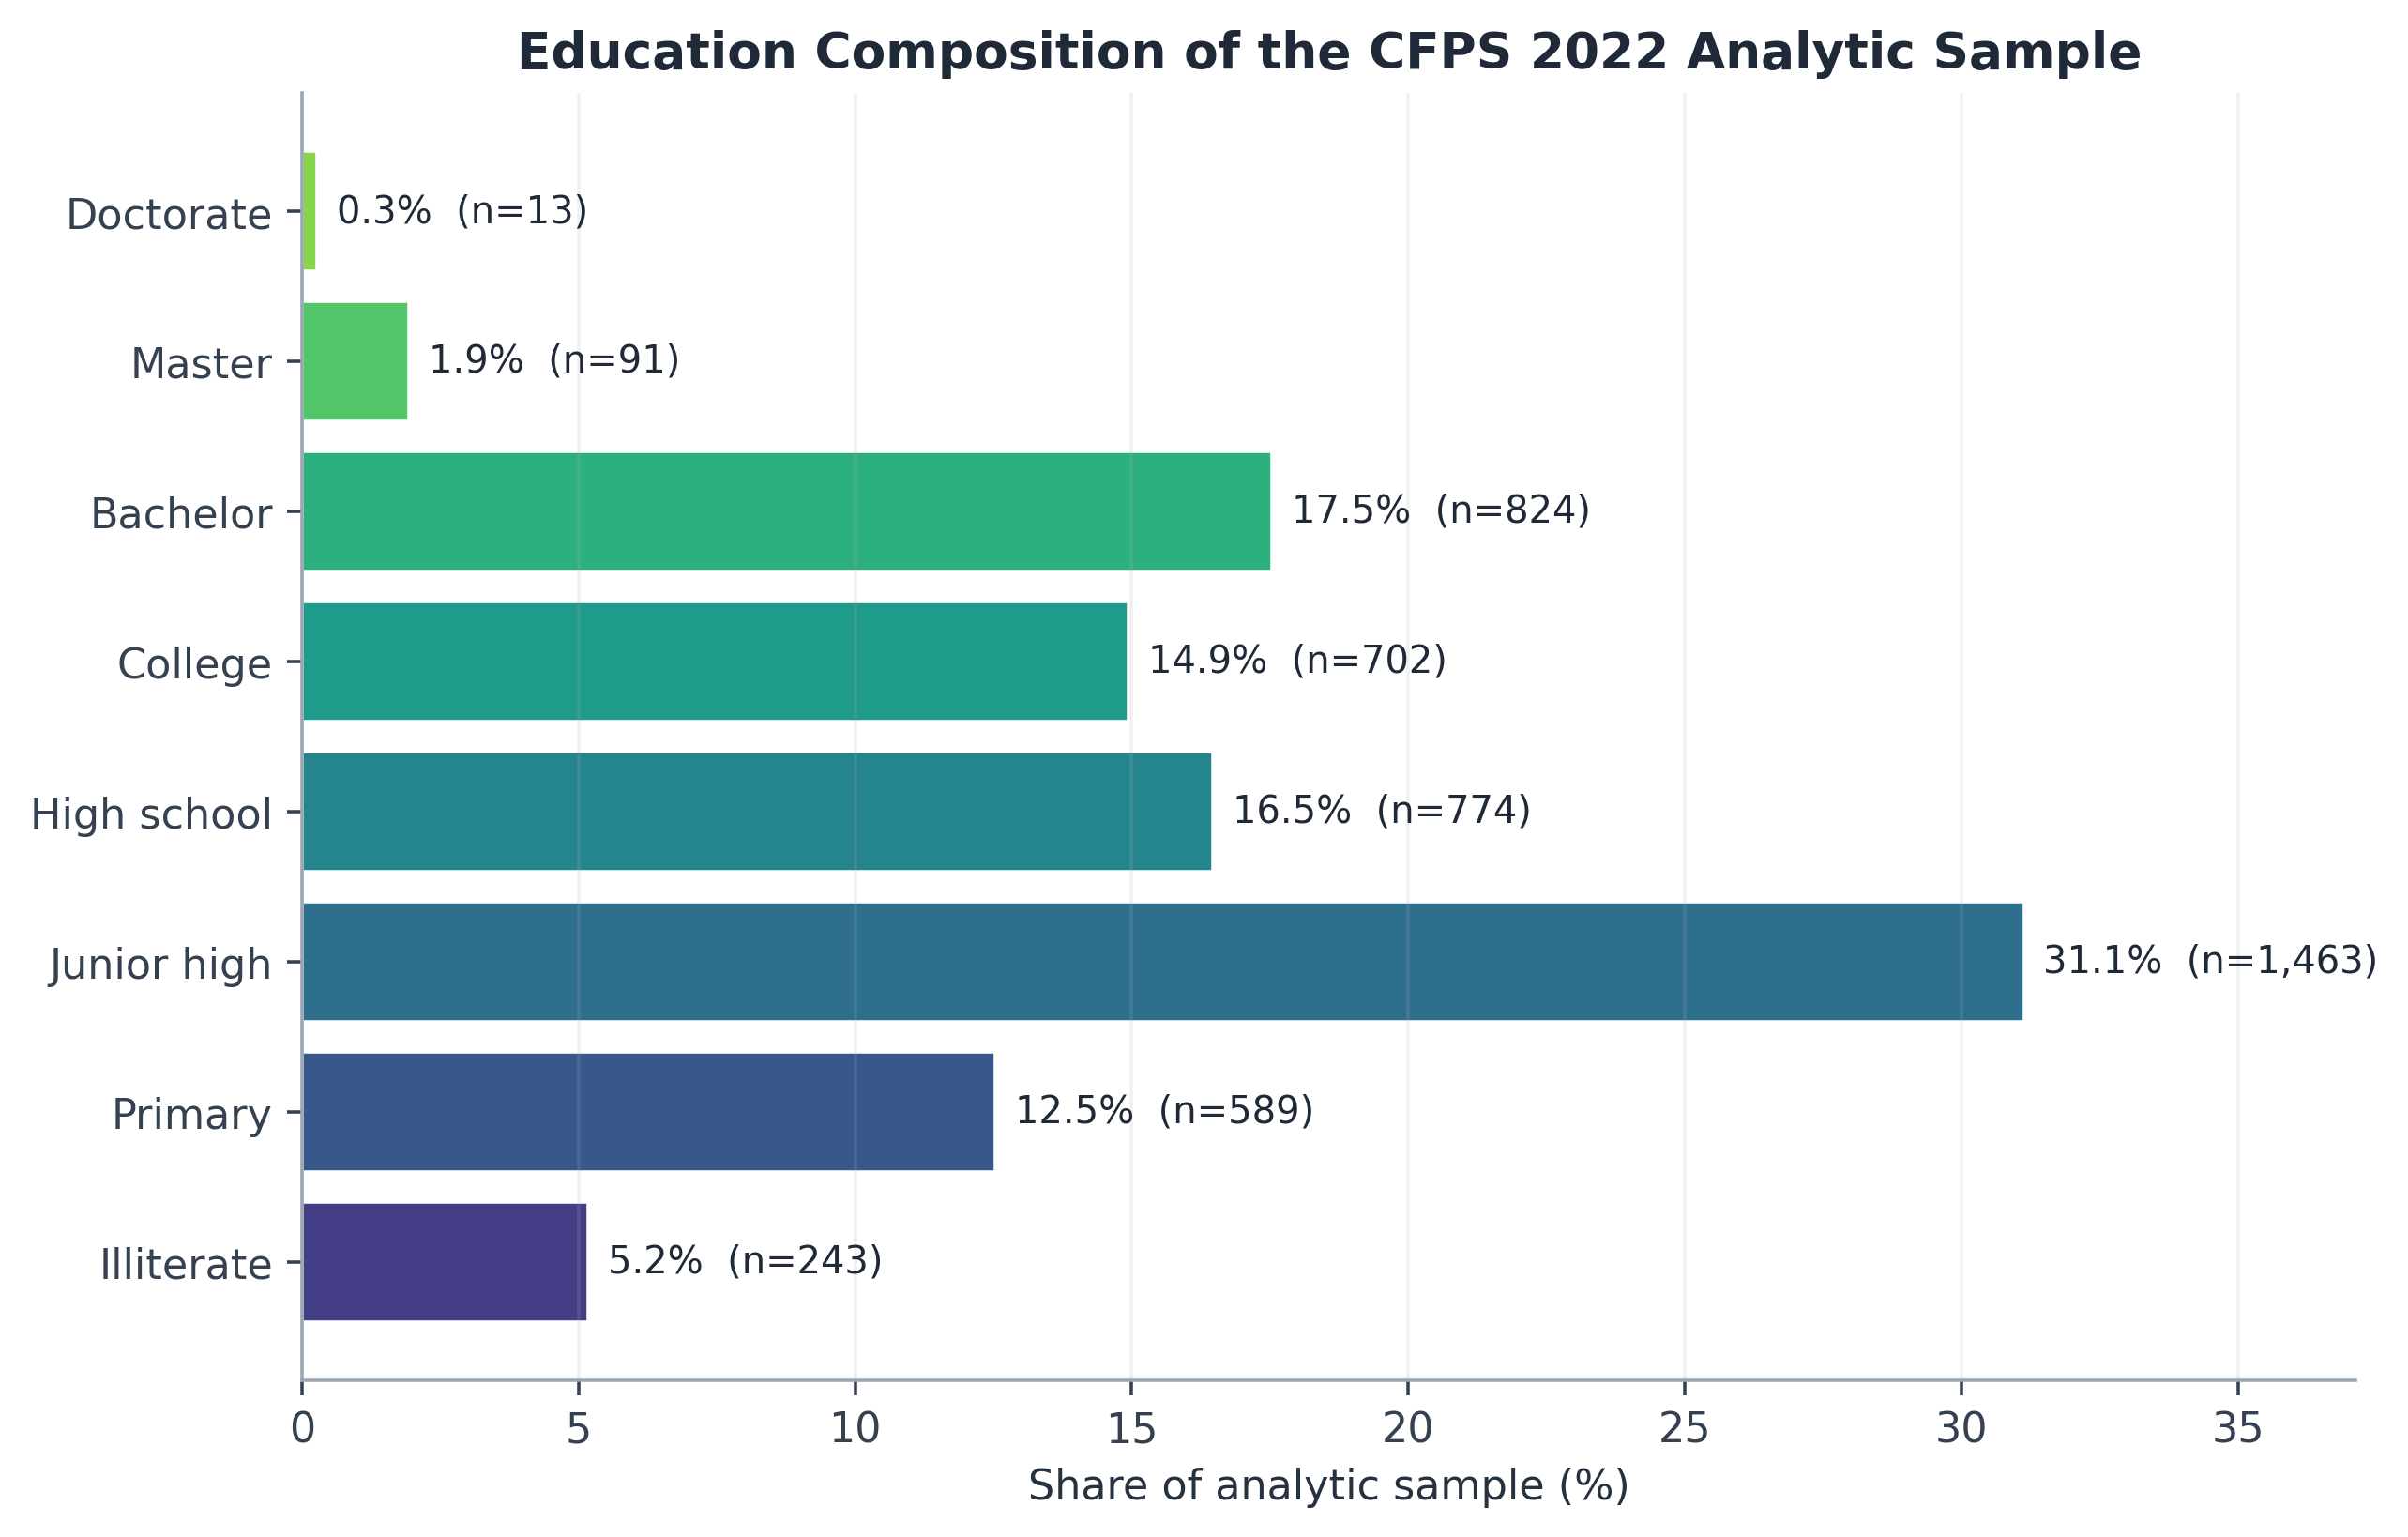
\includegraphics[width=0.86\textwidth]{figures/viz_education_distribution.png}
\caption{分析样本的教育构成}
\label{fig:education}
\end{figure}

\begin{figure}[H]
\centering
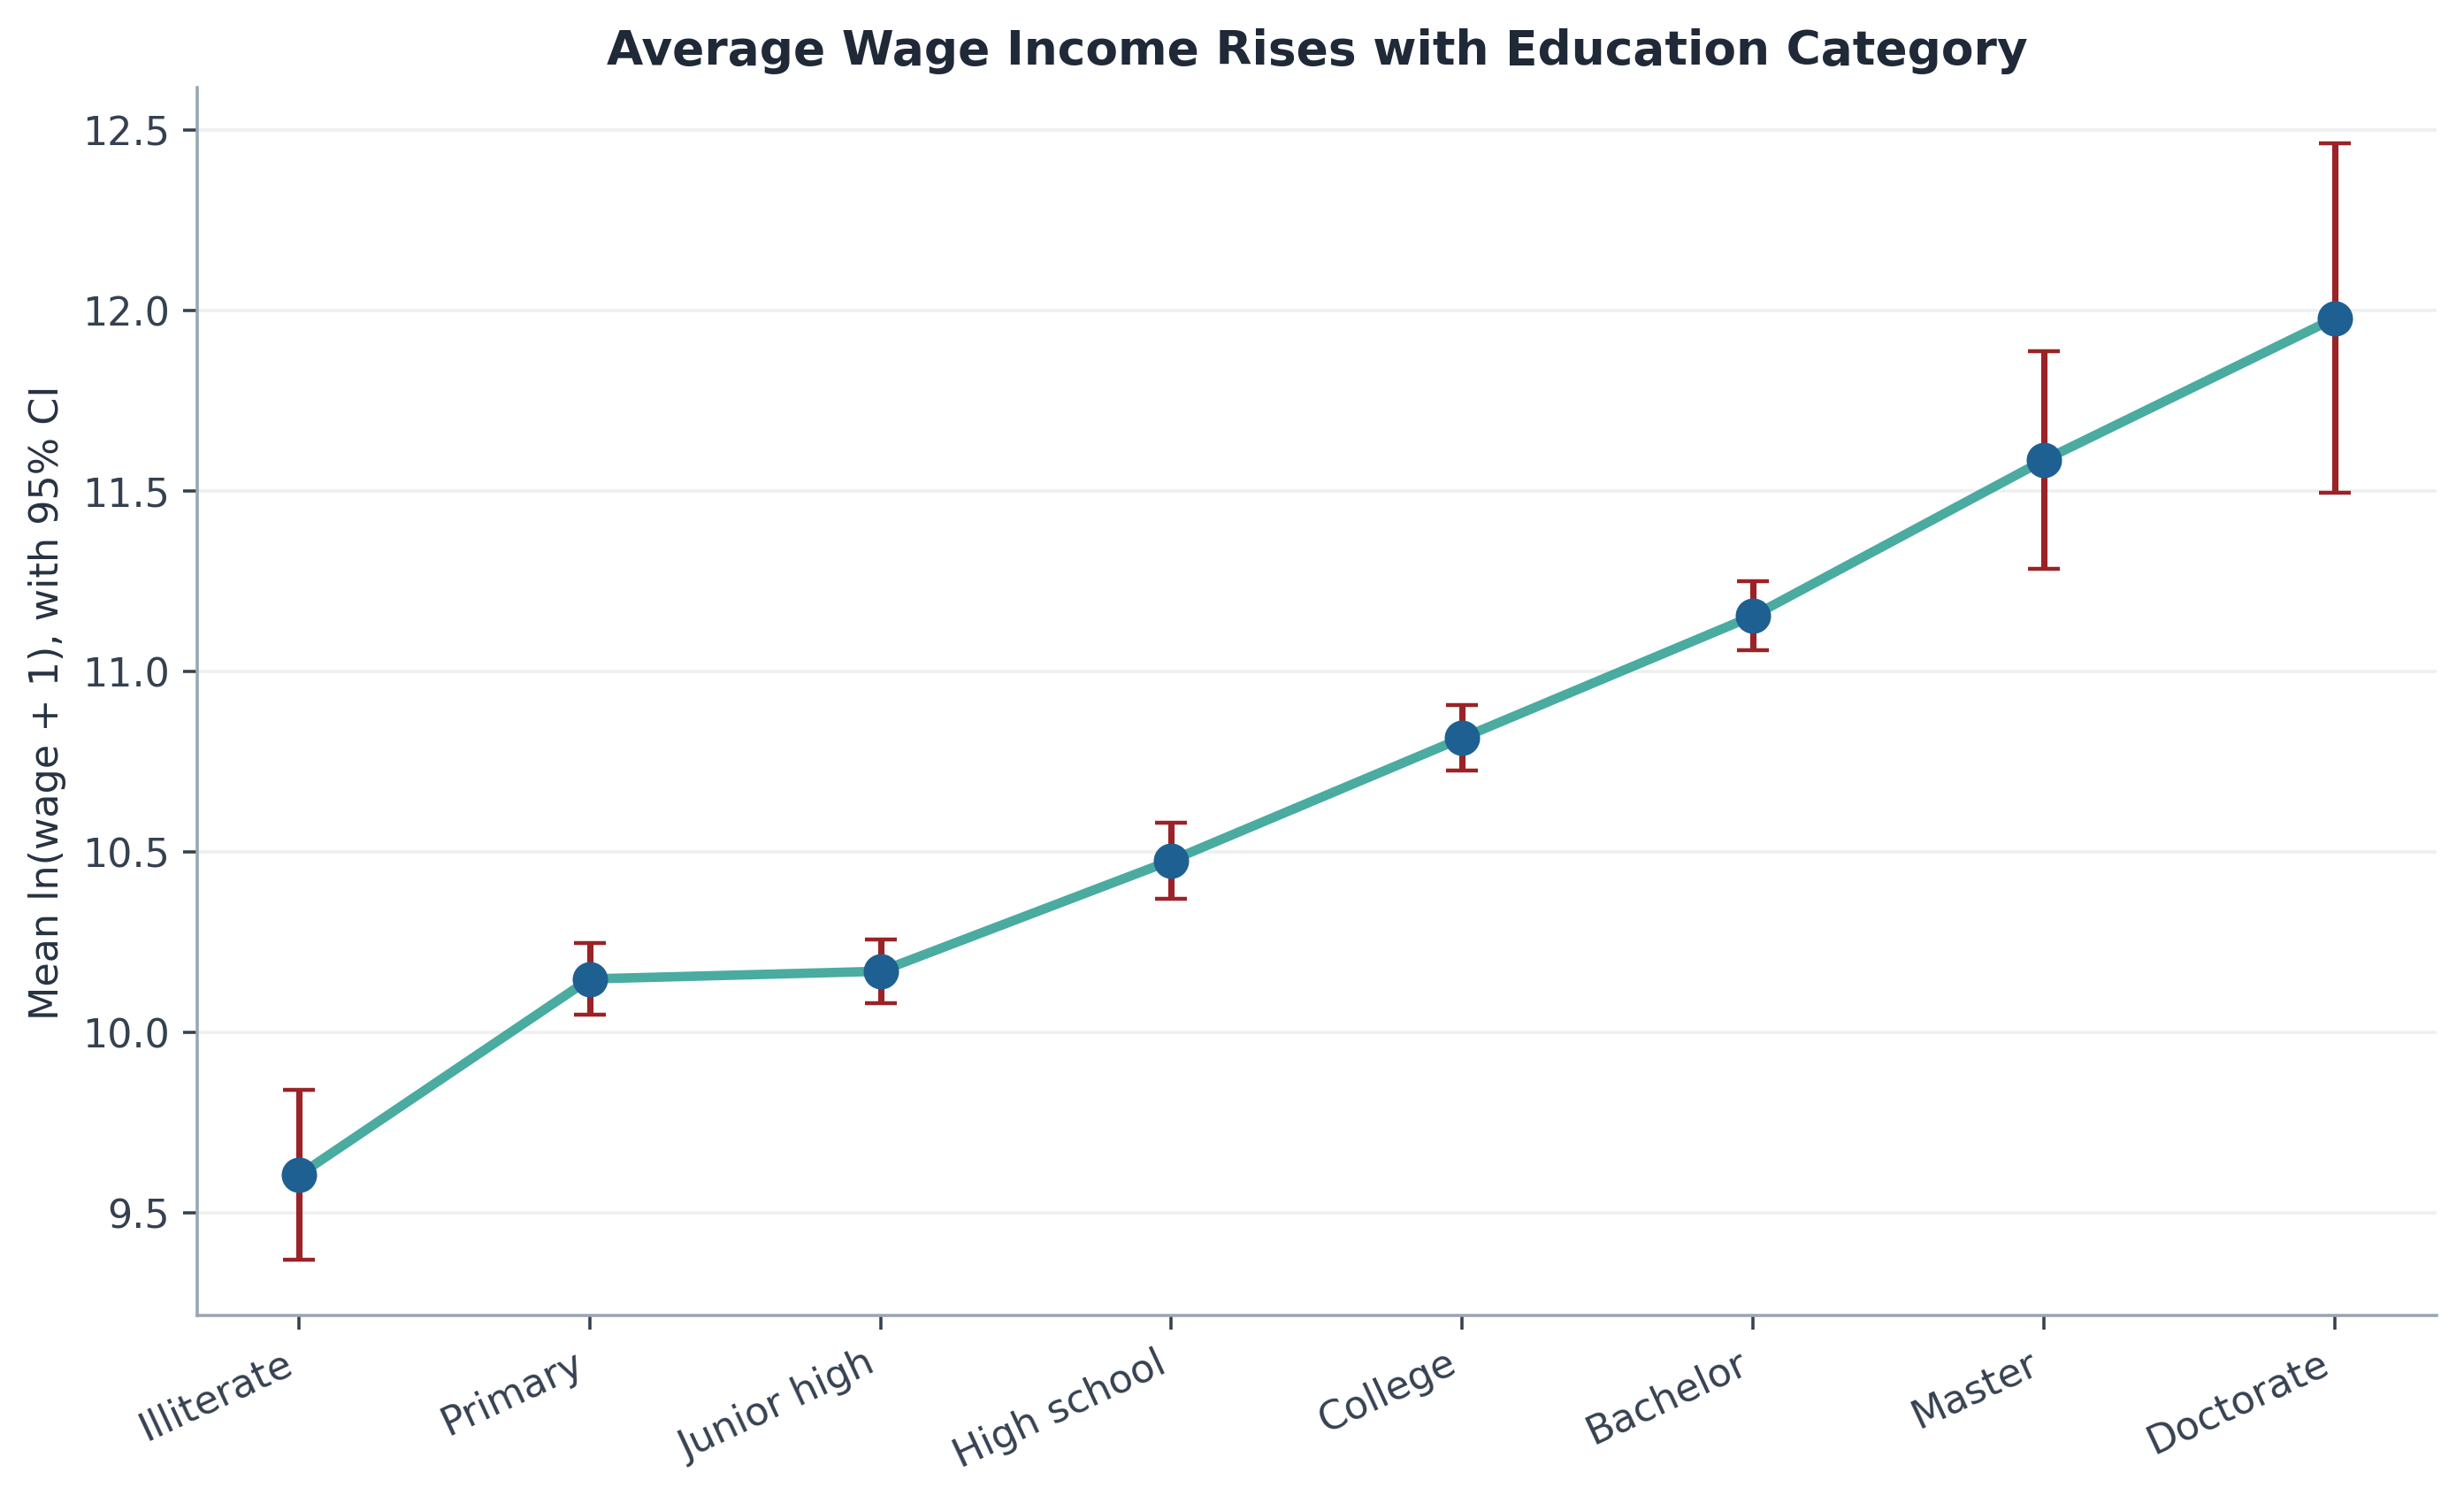
\includegraphics[width=0.86\textwidth]{figures/viz_wage_by_education.png}
\caption{不同教育水平的平均对数工资}
\label{fig:wageedu}
\end{figure}

\section{实证策略}

\subsection{OLS 基准模型}

基准模型为：
\begin{equation}
\ln(\mathrm{wage}_i+1)=\alpha+\beta E_i+\gamma X_i+\mu_p+\varepsilon_i,
\end{equation}
其中 $E_i$ 表示受教育年限或大专及以上教育，$X_i$ 为控制变量，$\mu_p$ 为省份固定效应。所有回归均使用稳健标准误。OLS 用作基准结果，但不直接解释为严格因果效应。

\subsection{双重稳健处理效应估计}

本文的核心估计量是大专及以上教育的平均处理效应：
\begin{equation}
ATE=E[Y_i(1)-Y_i(0)].
\end{equation}
AIPW 个体得分为：
\begin{equation}
\hat{\tau}_i =
\hat{m}_1(X_i)-\hat{m}_0(X_i)
+\frac{D_i(Y_i-\hat{m}_1(X_i))}{\hat{e}(X_i)}
-\frac{(1-D_i)(Y_i-\hat{m}_0(X_i))}{1-\hat{e}(X_i)},
\end{equation}
其中 $D_i$ 表示是否完成大专及以上教育，$\hat{e}(X_i)$ 为倾向得分，$\hat{m}_d(X_i)$ 为处理状态 $d$ 下的预测收入。本文使用五折交叉拟合，并同时报告线性模型和梯度提升模型。首选设定控制年龄、性别、户口、城乡、婚姻、医保和省份；扩展设定进一步加入健康、家庭规模、社会地位、是否上网和就业状态。

\subsection{扩招工具变量诊断}

1999 年中国高等教育扩招提供了一个潜在政策冲击。本文用出生年份减 1981 作为 running variable，因为 1981 年出生队列在 1999 年大约 18 岁。若该设计有效，1981 年及以后出生应在教育水平上出现局部跳跃。本文在多个对称出生队列窗口中报告第一阶段和 IV 估计，以判断这一识别策略是否足够强。

\section{实证结果}

\subsection{OLS 基准结果}

表 \ref{tab:reg} 显示，OLS 结果方向稳定。基础设定中，受教育年限系数为 0.088；加入更多控制变量后为 0.083。以大专及以上作为处理变量时，基础设定系数为 0.738，扩展设定为 0.694。

\begin{table}[H]
\centering
\caption{OLS 基准估计}
\label{tab:reg}
\begin{tabular}{lrrrr}
\toprule
模型 & 教育系数 & 稳健标准误 & 样本量 & $R^2$ \\
\midrule
模型 1 & 0.0996*** & (0.0052) & 4,699 & 0.077 \\
模型 2 & 0.0959*** & (0.0063) & 4,699 & 0.127 \\
模型 3 & 0.0882*** & (0.0062) & 4,699 & 0.158 \\
替代收入 & 0.0728*** & (0.0030) & 4,699 & 0.340 \\
正工资样本 & 0.0788*** & (0.0037) & 4,638 & 0.297 \\
\bottomrule
\end{tabular}

\begin{flushleft}
\footnotesize 注：括号内为稳健标准误。基础控制变量包括年龄、年龄平方、性别、婚姻、农业户口、医保和省份固定效应；扩展控制变量进一步加入城乡、健康、家庭规模、是否上网和主观社会地位。$^{*}p<0.10$，$^{**}p<0.05$，$^{***}p<0.01$。
\end{flushleft}
\end{table}

\begin{figure}[H]
\centering
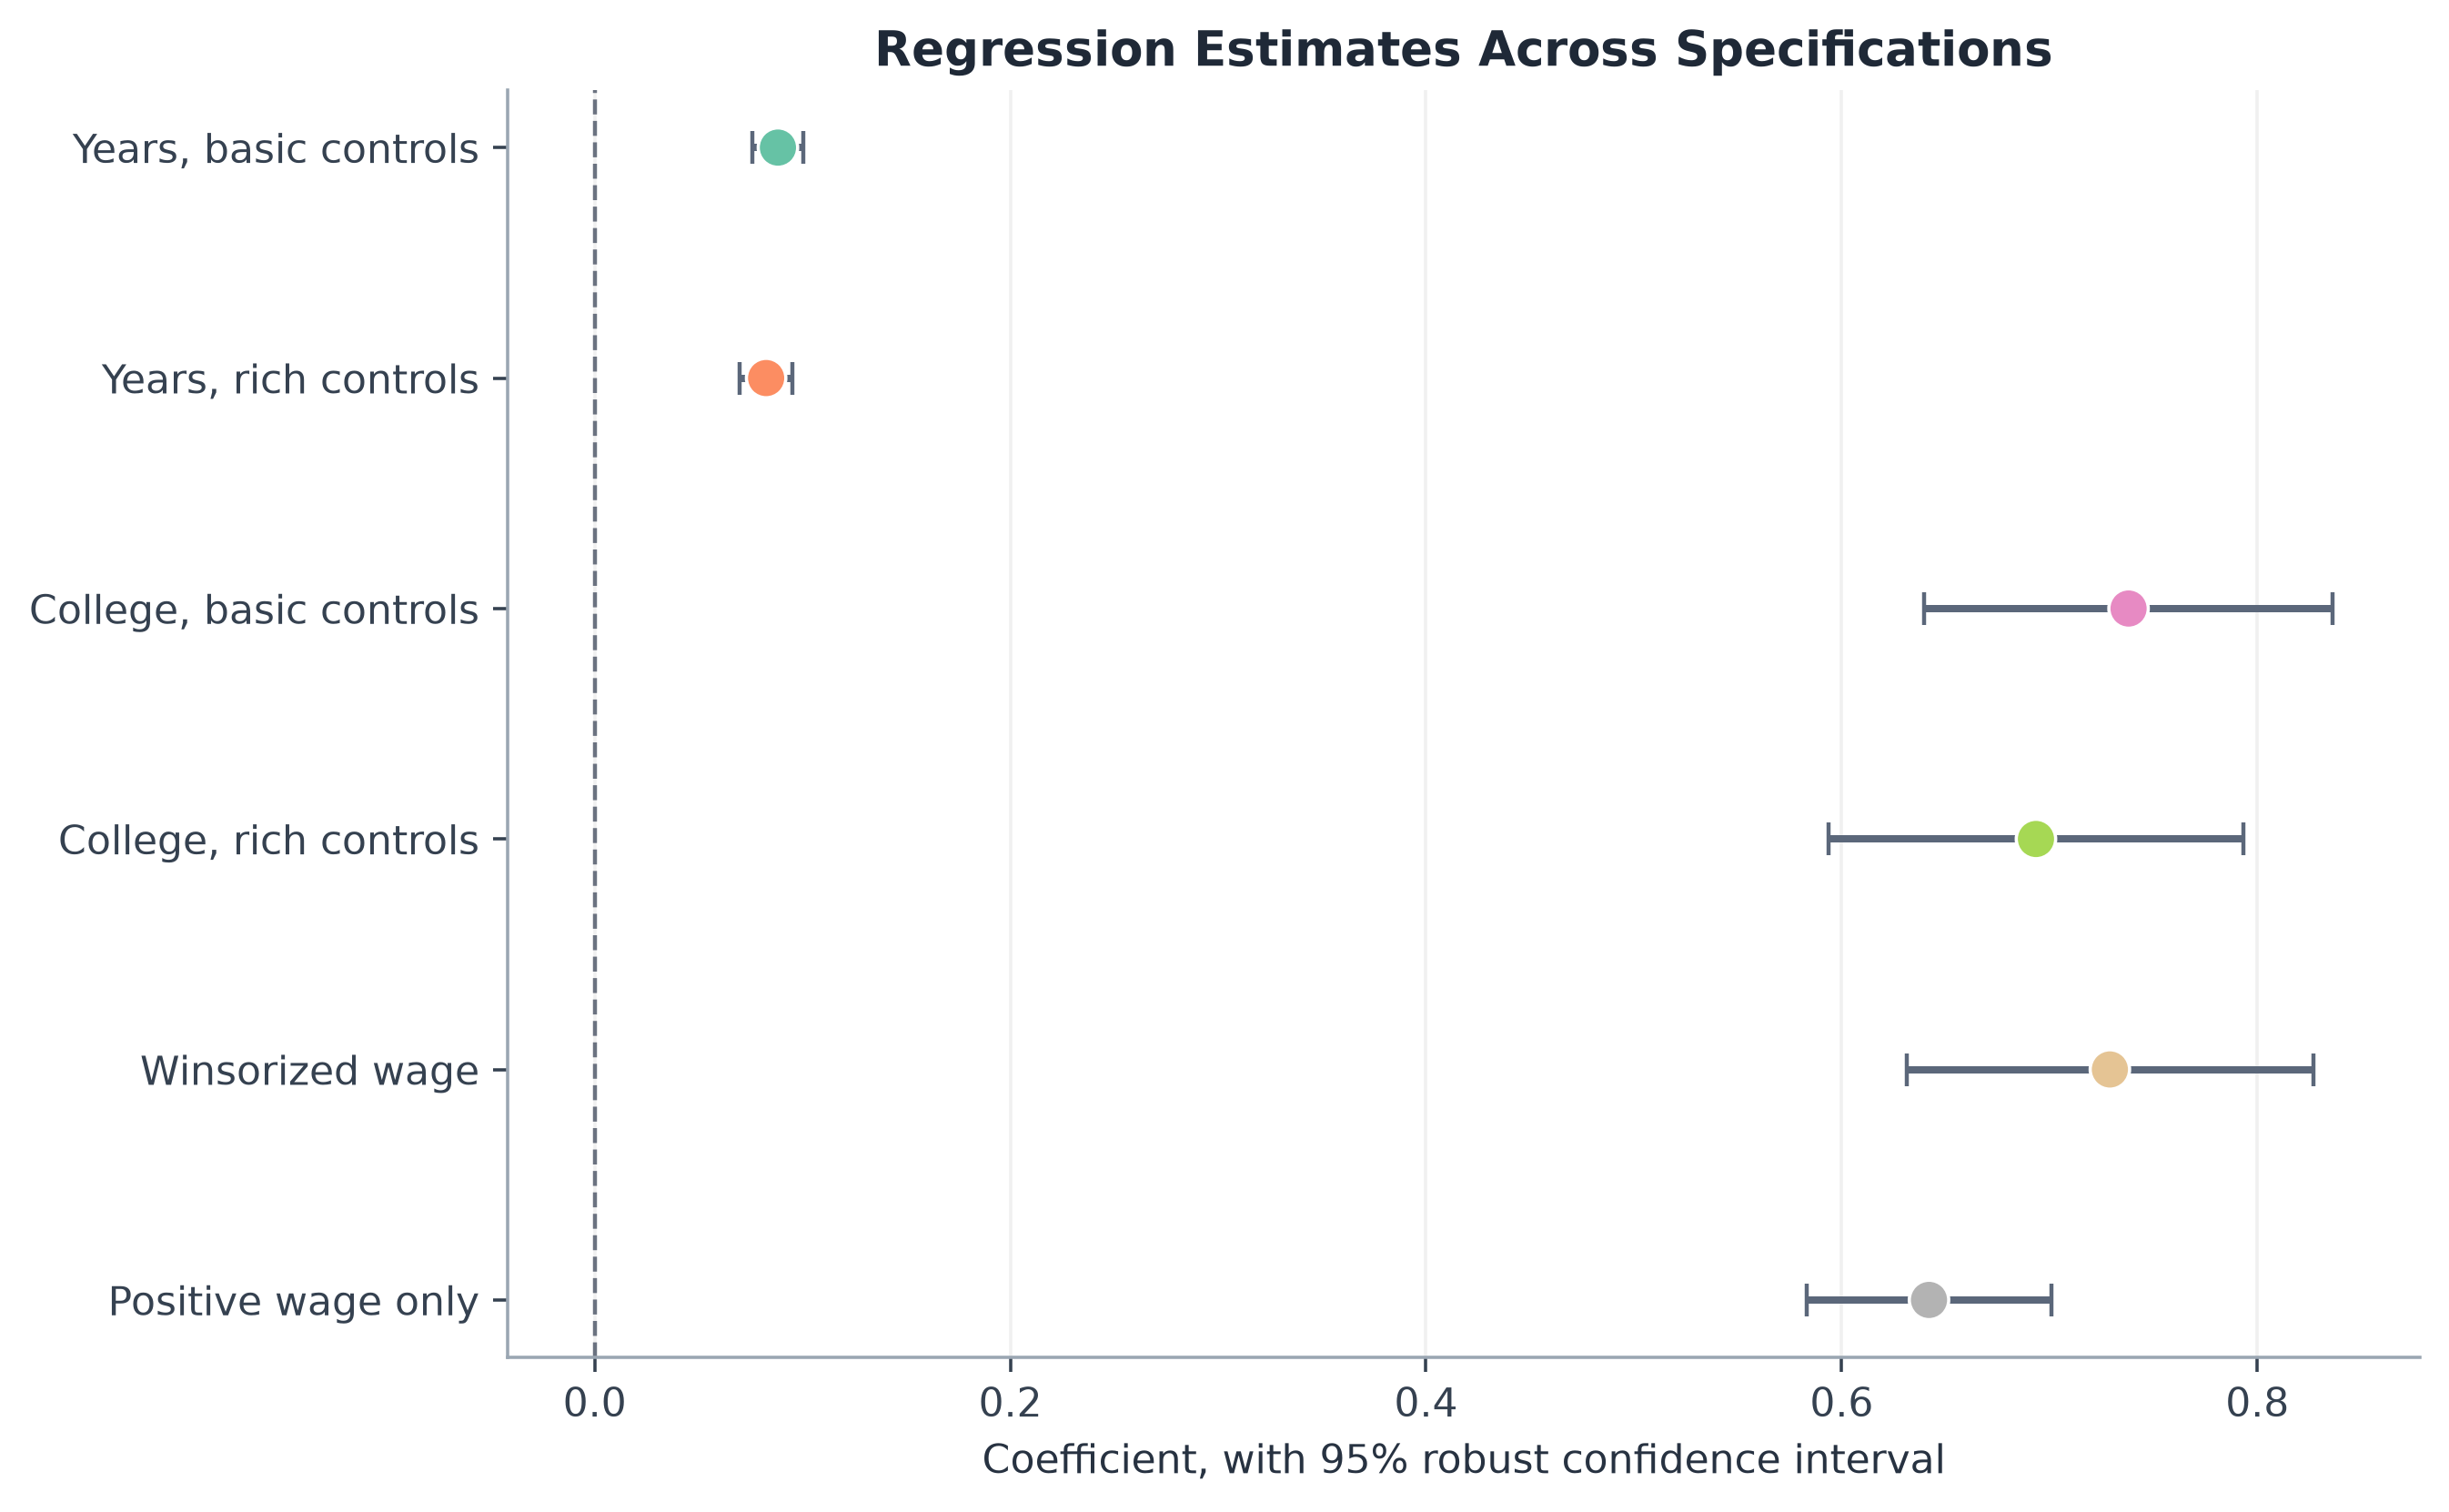
\includegraphics[width=0.86\textwidth]{figures/viz_regression_coefficients.png}
\caption{不同模型中的教育收入系数}
\label{fig:coef}
\end{figure}

\subsection{双重稳健估计}

表 \ref{tab:aipw} 报告 AIPW 结果。首选的 Core plus + GBM 估计为 0.710，标准误为 0.056。六组设定的估计范围为 0.669--0.773，说明结果并不依赖单一协变量组合或单一学习器。

\begin{table}[H]
\centering
\caption{大专及以上教育的 AIPW 估计}
\label{tab:aipw}
\begin{tabular}{llrrlrr}
\toprule
协变量 & 学习器 & ATE & 标准误 & 95\% CI & 样本量 & AUC \\
\midrule
Core & Linear & 0.7726*** & (0.0551) & [0.6647, 0.8806] & 4,699 & 0.814 \\
Core & GBM & 0.7206*** & (0.0553) & [0.6123, 0.8289] & 4,699 & 0.822 \\
Core plus & Linear & 0.7730*** & (0.0548) & [0.6655, 0.8804] & 4,699 & 0.813 \\
Core plus & GBM & 0.7154*** & (0.0570) & [0.6038, 0.8270] & 4,699 & 0.824 \\
Extended & Linear & 0.7203*** & (0.0517) & [0.6190, 0.8216] & 4,699 & 0.827 \\
Extended & GBM & 0.6859*** & (0.0489) & [0.5901, 0.7817] & 4,699 & 0.843 \\
\bottomrule
\end{tabular}

\begin{flushleft}
\footnotesize 注：因变量为 $\ln(\mathrm{wage}+1)$。ATE 表示完成大专及以上教育的平均处理效应。Linear 使用逻辑回归/Ridge 结果模型；GBM 使用梯度提升模型。首选设定为 Core plus + GBM。
\end{flushleft}
\end{table}

AIPW 的可信度取决于共同支撑和平衡性。图 \ref{fig:propensity} 显示处理组和对照组在较宽的倾向得分区间内存在重叠，但两端仍有少量样本。表 \ref{tab:balance} 和图 \ref{fig:balance} 显示，加权后核心协变量的标准化差异绝对值均降至 0.10 以下。

\begin{figure}[H]
\centering
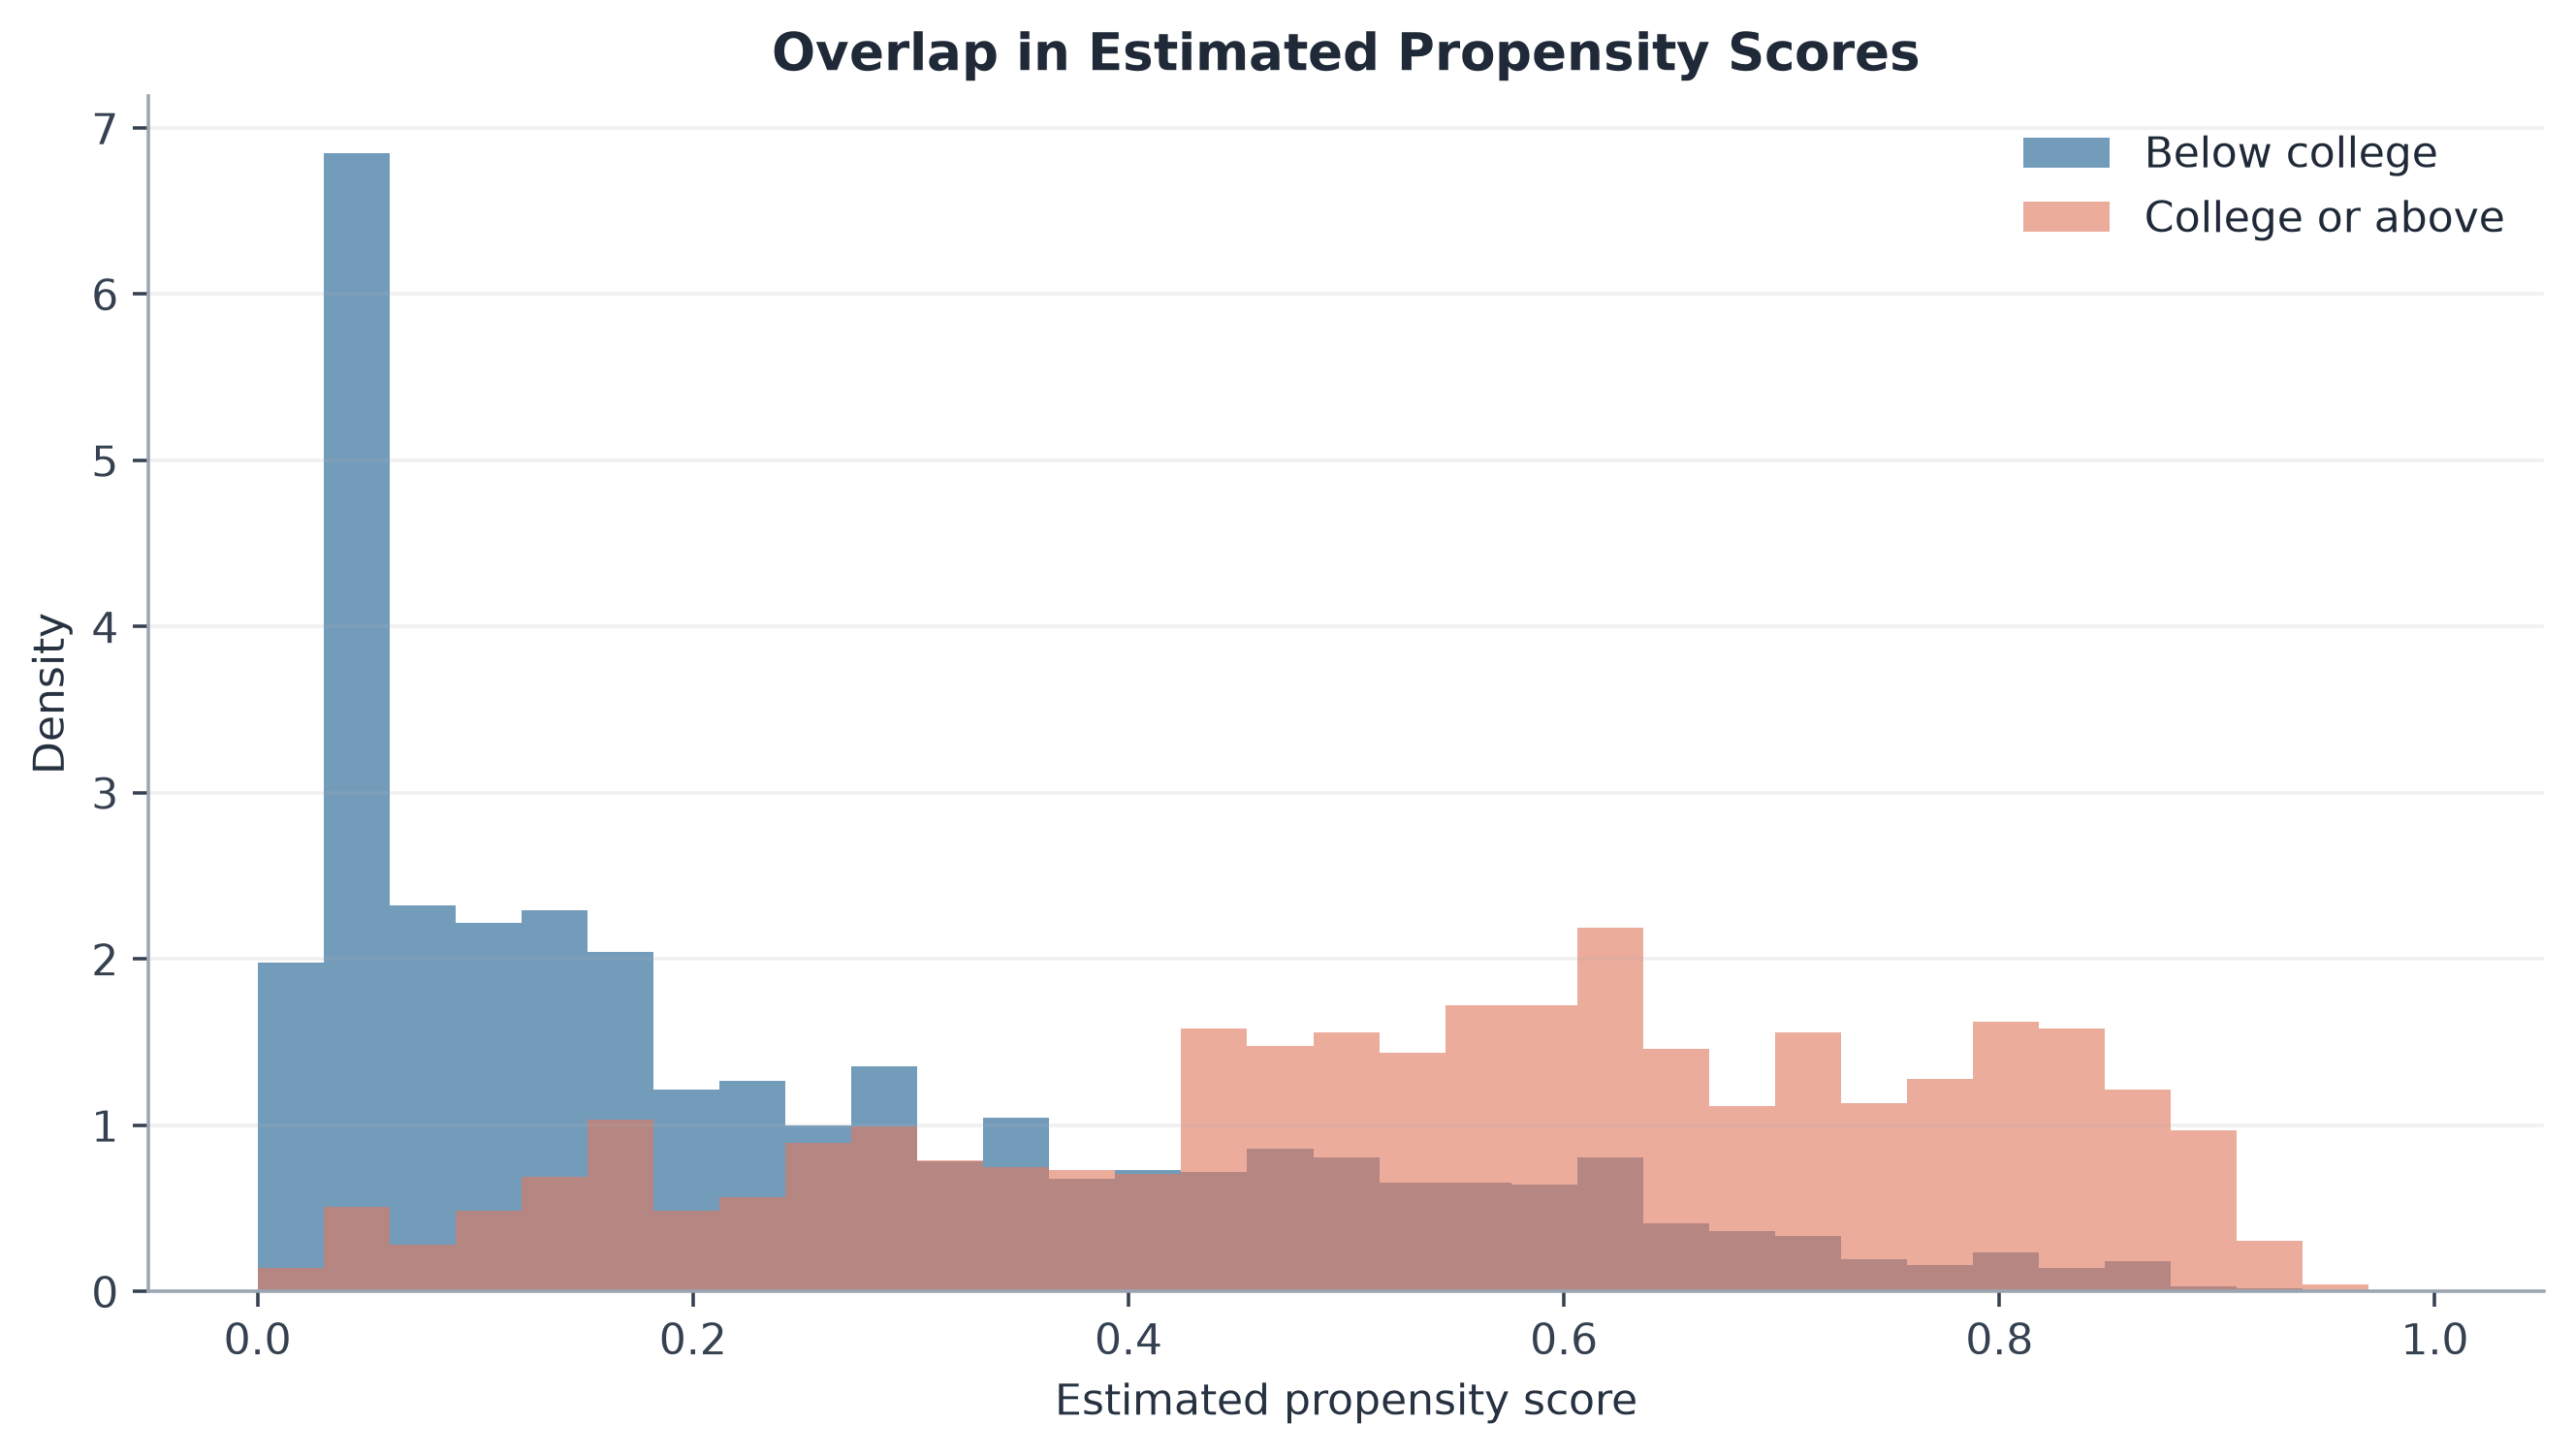
\includegraphics[width=0.86\textwidth]{figures/viz_propensity_overlap.png}
\caption{倾向得分共同支撑}
\label{fig:propensity}
\end{figure}

\begin{table}[H]
\centering
\caption{加权前后的协变量平衡性}
\label{tab:balance}
\begin{tabular}{lrr}
\toprule
协变量 & 原始 SMD & 加权 SMD \\
\midrule
age\_ & -0.937 & -0.069 \\
gen & -0.214 & 0.037 \\
rural & -0.525 & -0.021 \\
urban & 0.642 & 0.029 \\
mar & -0.286 & -0.026 \\
\bottomrule
\end{tabular}

\end{table}

\begin{figure}[H]
\centering
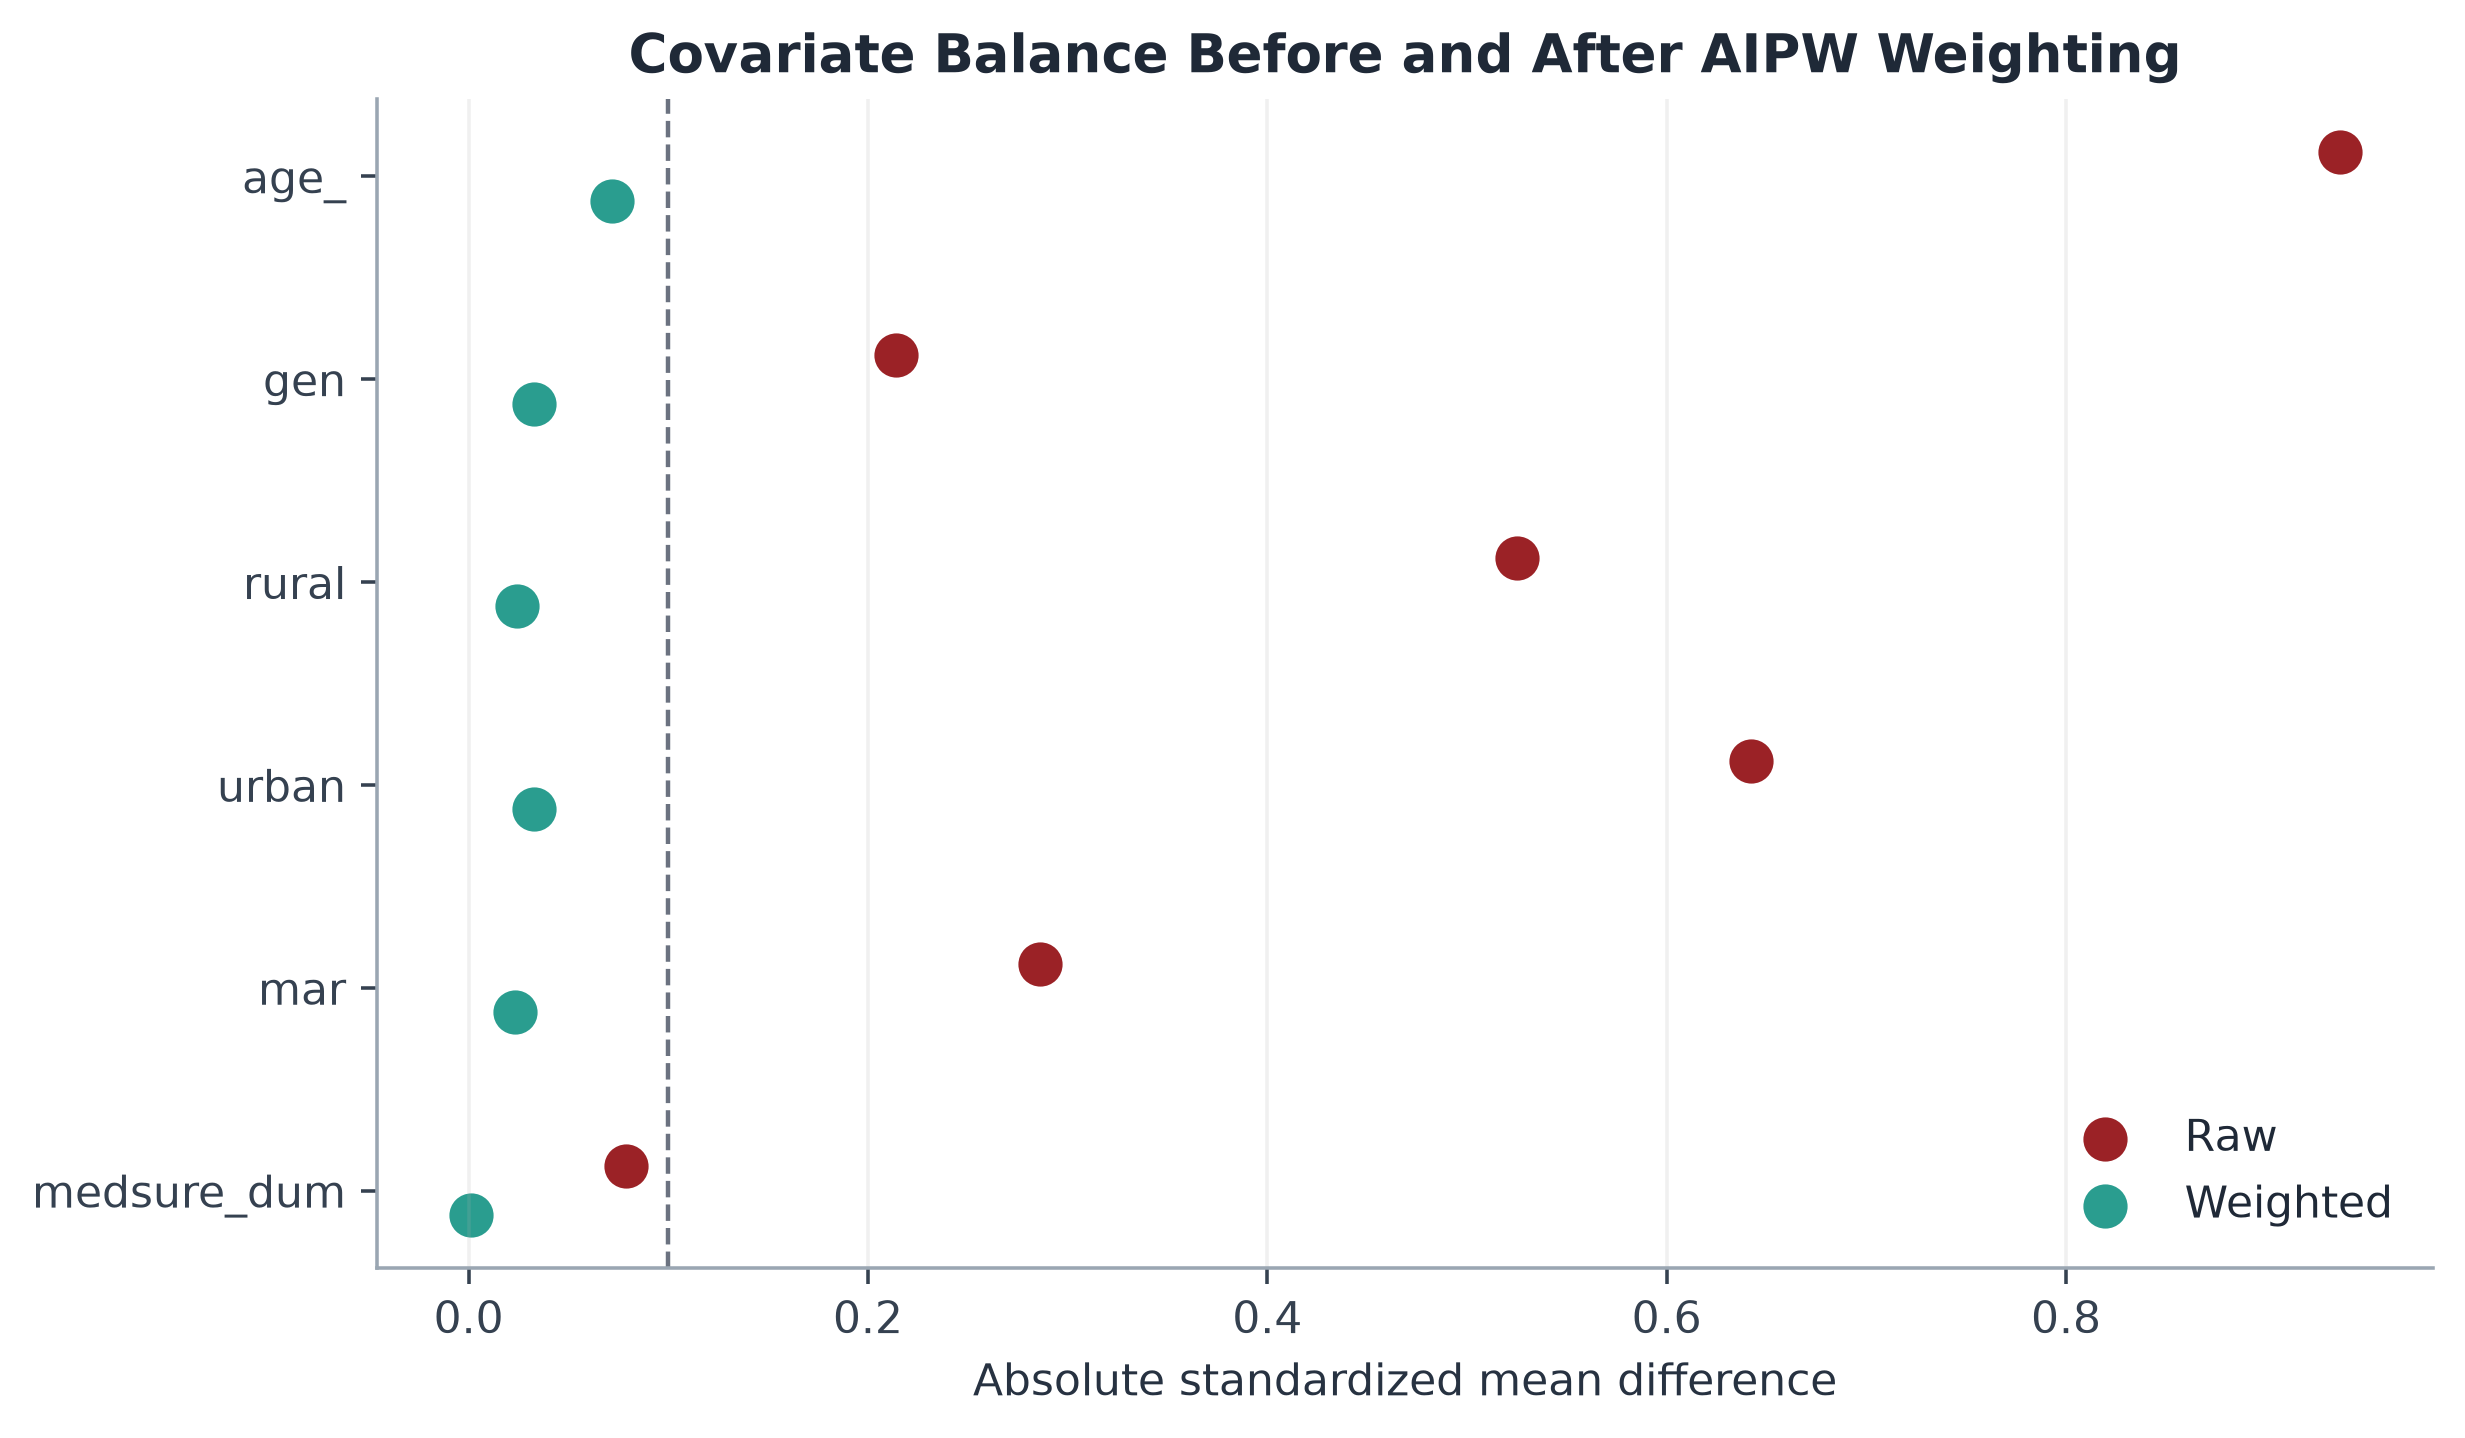
\includegraphics[width=0.80\textwidth]{figures/viz_balance_diagnostics.png}
\caption{加权前后的标准化均值差异}
\label{fig:balance}
\end{figure}

\subsection{弱工具变量诊断}

图 \ref{fig:cohort} 展示 1981 年 cutoff 附近出生队列的大专及以上比例和平均教育年限。表 \ref{tab:iv} 显示，在 $\pm 5$ 到 $\pm 15$ 年的较窄窗口中，第一阶段 F 统计量远低于常用弱工具变量阈值。$\pm 20$ 年窗口的第一阶段较强，但窗口过宽，已经难以解释为局部断点。因此，扩招 IV 不作为本文主要因果证据。

\begin{figure}[H]
\centering
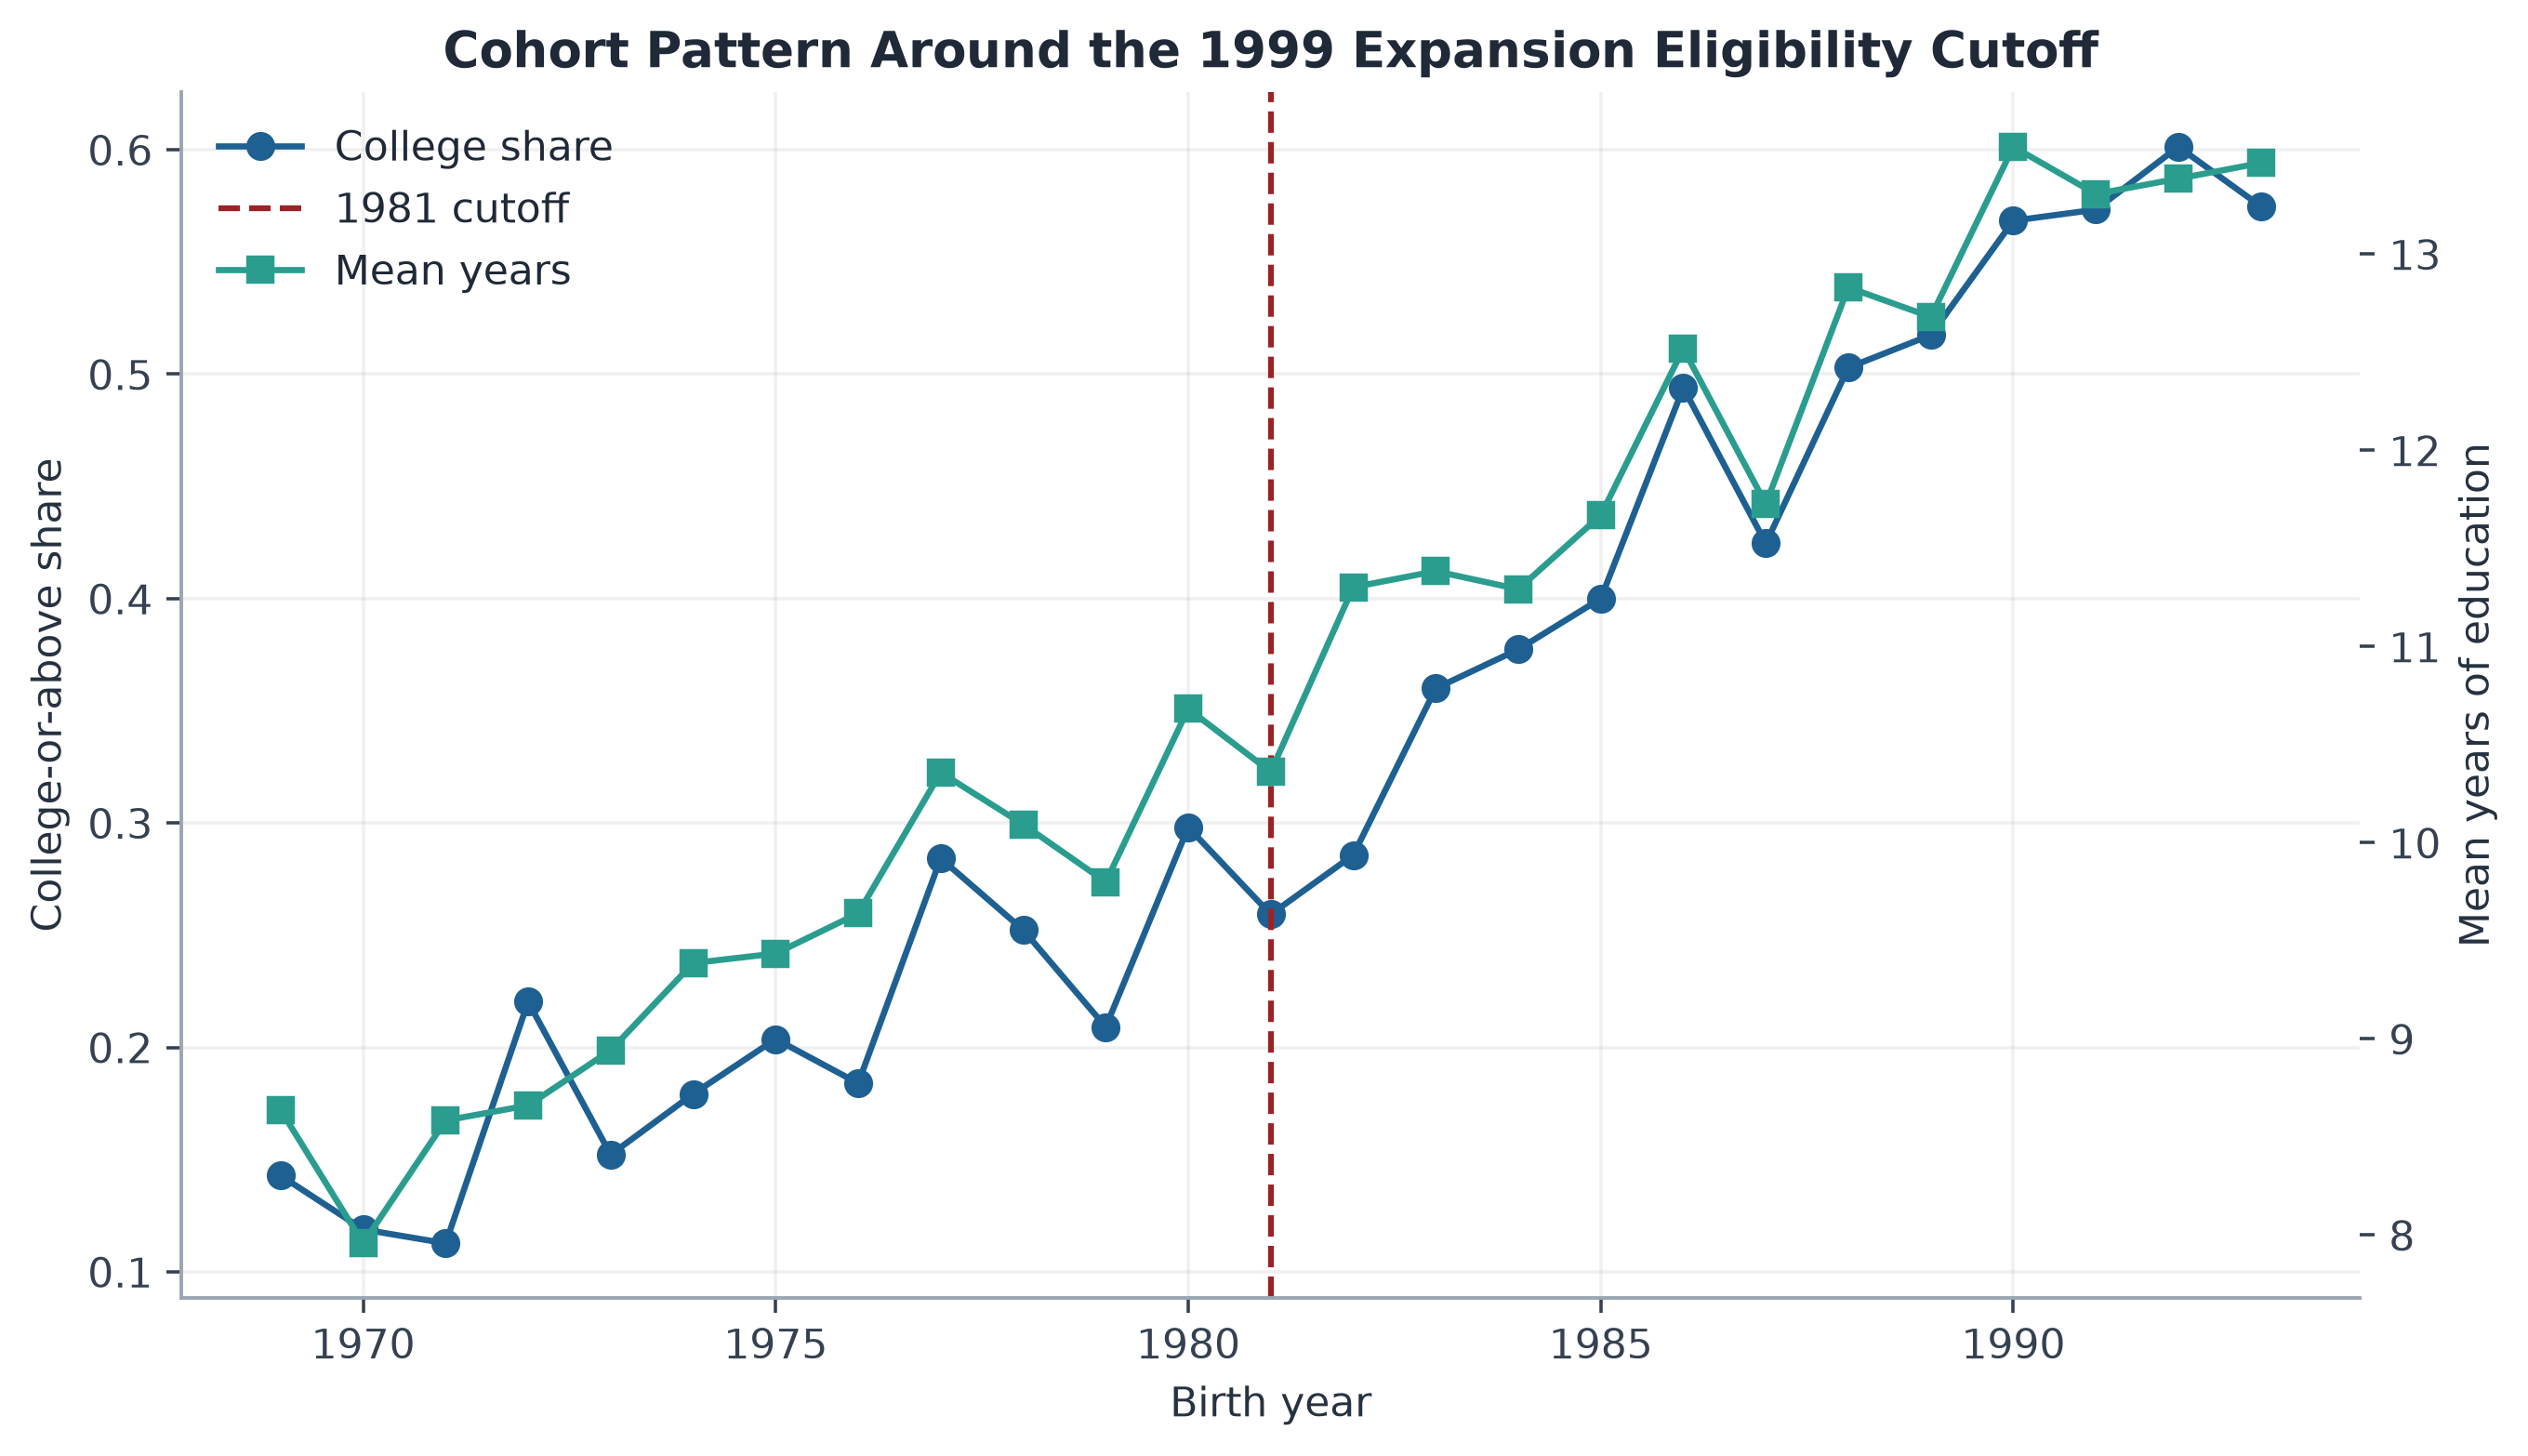
\includegraphics[width=0.86\textwidth]{figures/viz_cohort_first_stage.png}
\caption{高等教育扩招 cutoff 附近的出生队列模式}
\label{fig:cohort}
\end{figure}

\begin{table}[H]
\centering
\caption{高等教育扩招 IV 诊断}
\label{tab:iv}
\begin{tabular}{lrrrrr}
\toprule
窗口 & 样本量 & 第一阶段 & F 统计量 & IV 估计 & 标准误 \\
\midrule
+/-5 & 1,280 & -0.0743 & 0.03 & 0.5195 & (3.2703) \\
+/-7 & 1,844 & 0.1961 & 0.29 & 0.4589 & (0.9572) \\
+/-9 & 2,462 & -0.0481 & 0.02 & 0.2091 & (2.4996) \\
+/-12 & 3,277 & 0.1269 & 0.21 & -0.7816 & (2.0357) \\
+/-15 & 3,933 & 0.3977 & 2.54 & -0.1531 & (0.2721) \\
+/-20 & 4,596 & 1.2985 & 33.22 & 0.0414 & (0.0633) \\
\bottomrule
\end{tabular}

\begin{flushleft}
\footnotesize 注：工具变量为是否出生于 1981 年及以后，并控制线性 running variable、交互项和省份固定效应。较窄窗口中的第一阶段较弱，因此 IV 结果不应被解释为主要因果证据。
\end{flushleft}
\end{table}

\subsection{异质性}

表 \ref{tab:heterogeneity} 和图 \ref{fig:heterogeneity} 显示，女性样本中的教育系数高于男性，非农业户口样本中的教育系数高于农业户口样本。这与中国教育回报存在性别、户口、部门和地区差异的既有文献相一致 \citep{ma2021meta, li2025gender}。

\begin{table}[H]
\centering
\caption{不同子样本中的教育系数}
\label{tab:heterogeneity}
\begin{tabular}{lrrrr}
\toprule
子样本 & 教育系数 & 稳健标准误 & 样本量 & $R^2$ \\
\midrule
女性 & 0.1098*** & (0.0091) & 1,996 & 0.155 \\
男性 & 0.0671*** & (0.0067) & 2,703 & 0.145 \\
非农业户口 & 0.1469*** & (0.0198) & 962 & 0.144 \\
农业户口 & 0.0774*** & (0.0064) & 3,737 & 0.128 \\
\bottomrule
\end{tabular}

\end{table}

\begin{figure}[H]
\centering
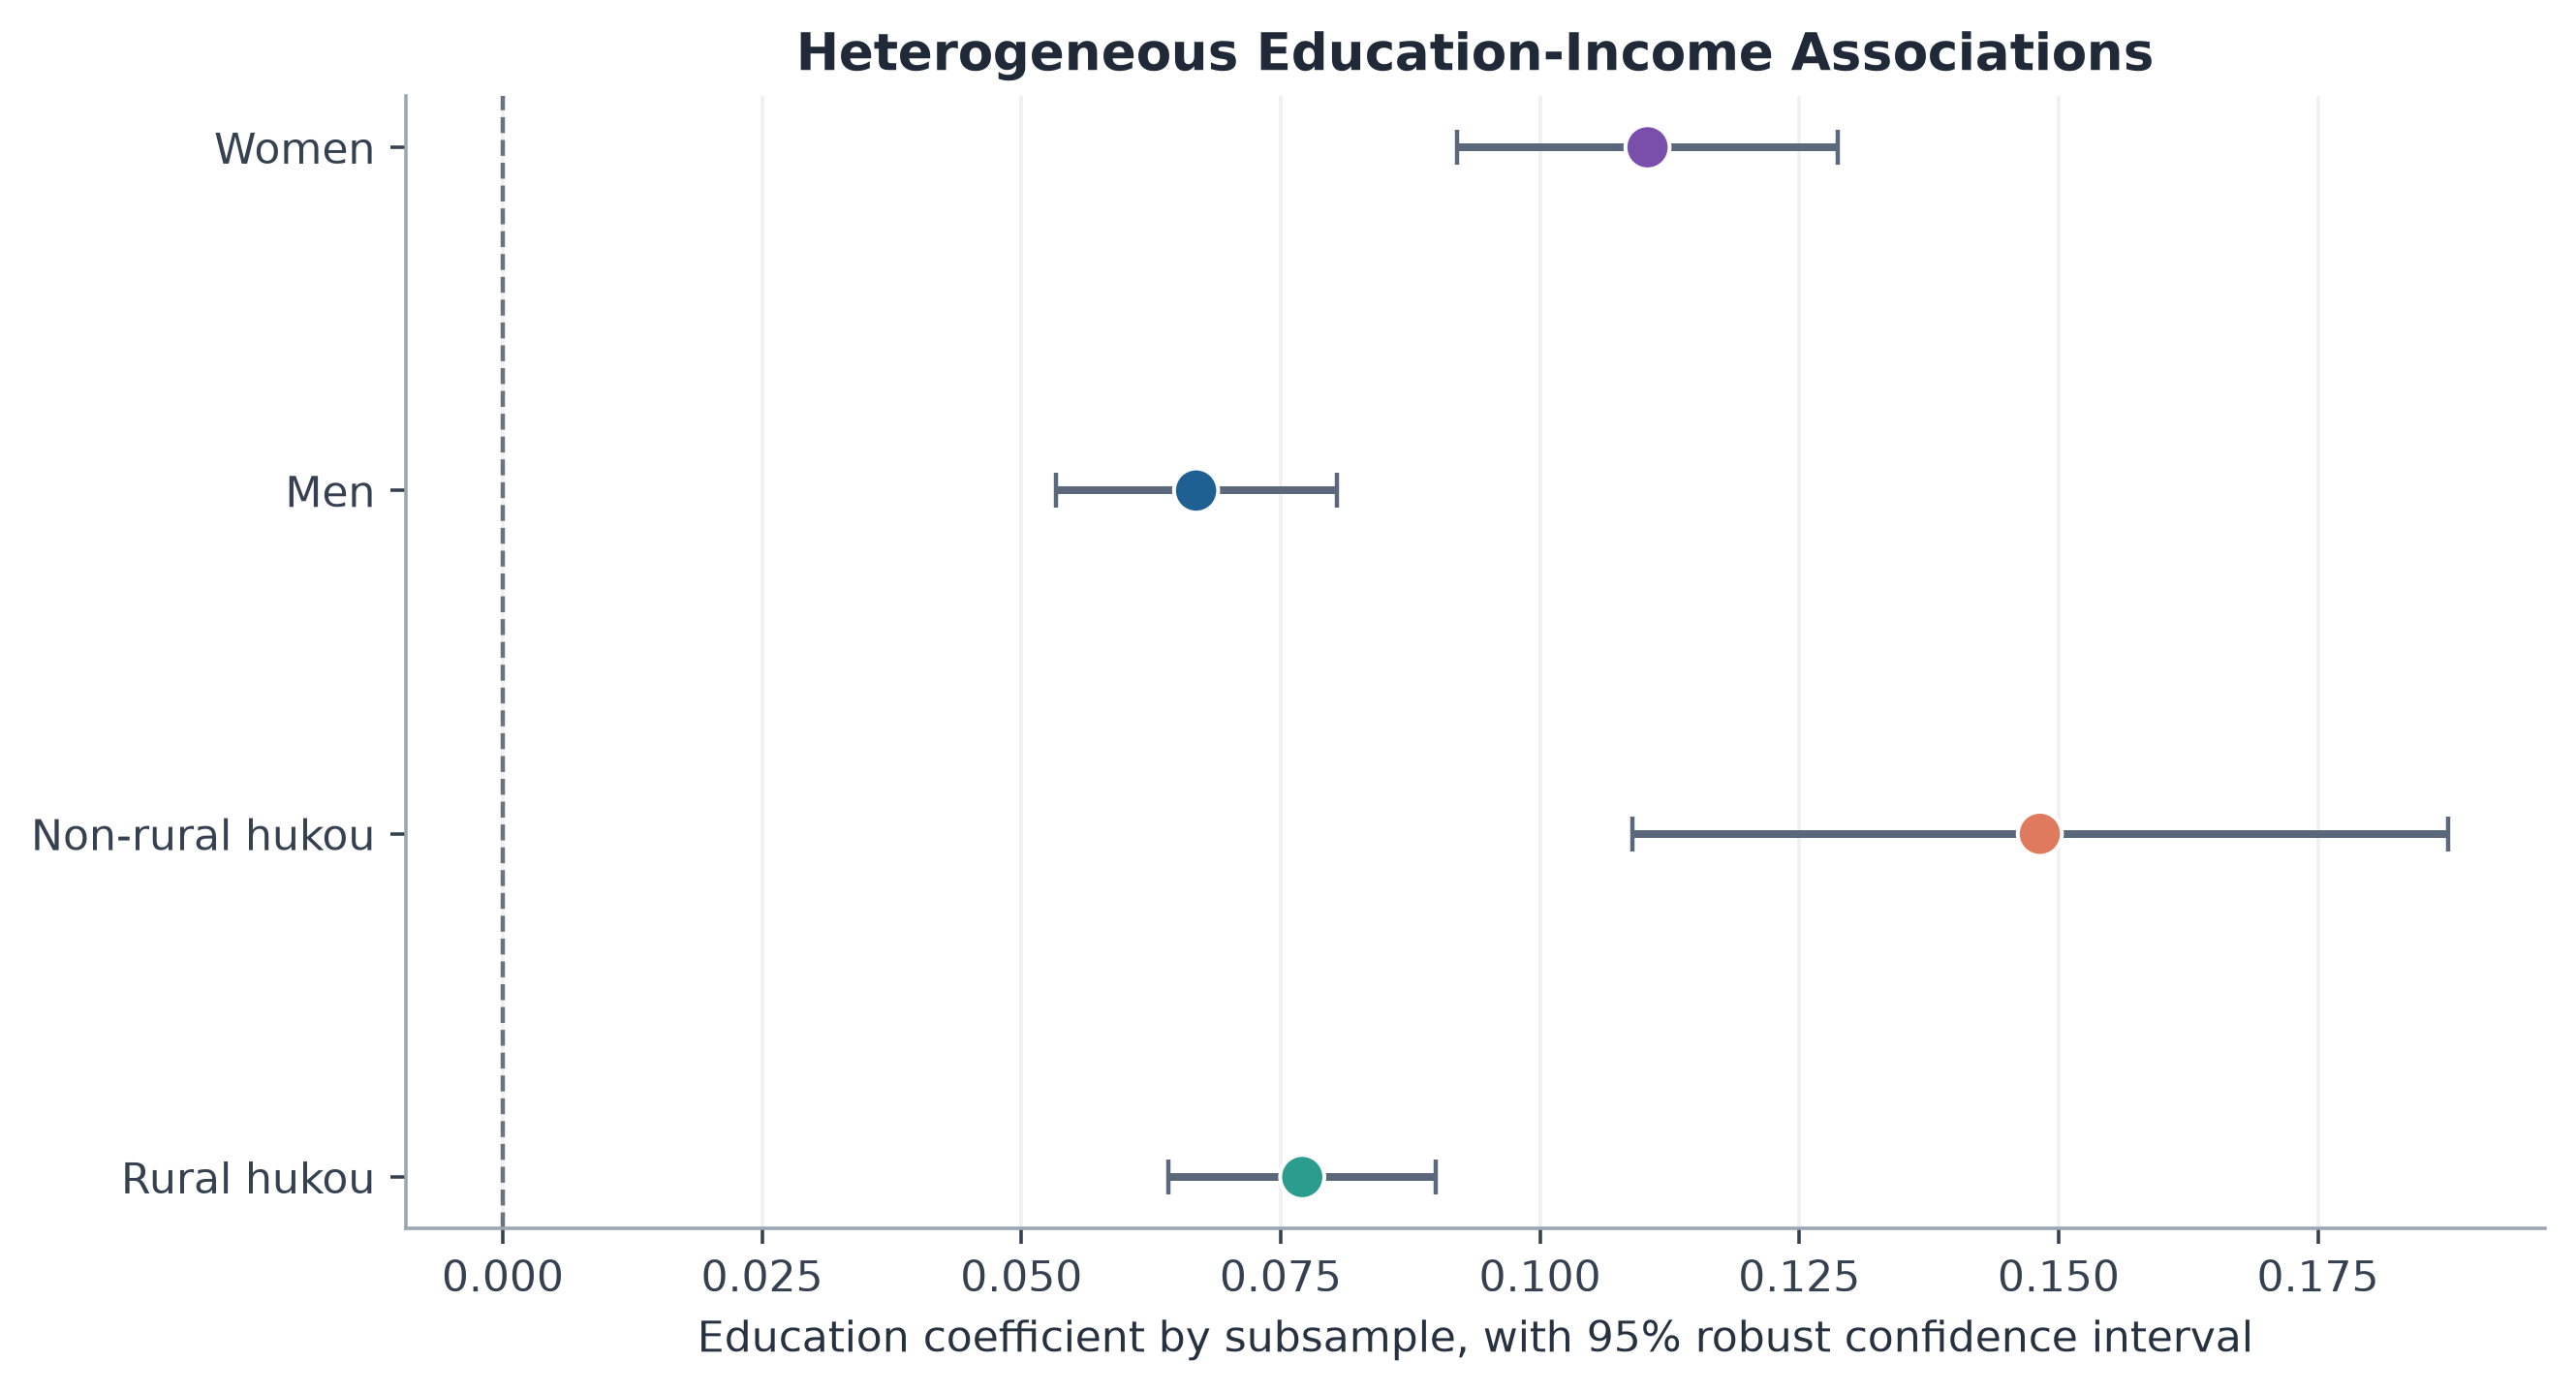
\includegraphics[width=0.82\textwidth]{figures/viz_heterogeneity_coefficients.png}
\caption{性别与户口子样本中的教育收入系数}
\label{fig:heterogeneity}
\end{figure}

\section{讨论}

新版实证相较于简单 OLS 有三点实质改进。第一，本文直接报告样本筛选和缺失情况，避免只展示最终回归样本。第二，本文将研究对象从“每增加一年教育”的相关关系扩展为“大专及以上教育”的处理效应，并使用双重稳健估计。第三，本文尝试政策型识别，但根据弱工具变量诊断保留谨慎解释，而不是为了创新而强行声称因果识别成功。

本文仍有局限。AIPW 依赖可观测变量调整，而当前数据文件缺少能力、父母教育、童年家庭资源和学校质量等重要变量。因此，首选估计应理解为选择性可观测条件下的双重稳健处理效应，而不是完全等同于随机实验或强工具变量估计。扩招 IV 的弱第一阶段也说明，仅凭当前横截面数据不宜做过强的政策因果结论。

\section{结论}

基于 CFPS 2022，本文发现教育与中国成年人收入之间存在显著正向关系。传统明瑟模型中，受教育年限每增加一年，工资收入约高 8.8\%。更重要的是，AIPW 结果显示，在平衡可观测协变量后，大专及以上教育对应约 0.71 个对数点的工资收入优势。该结果在不同协变量口径和学习器下保持稳定，且加权后协变量平衡明显改善。本文因此提供了一份比单纯 OLS 更有创新性、实证更扎实、并明确做过数据检查的教育收入研究。

\bibliographystyle{plainnat}
\bibliography{references}

\end{document}
